\section{Theorie}
\label{sec:Theorie}
\subsection{Geschichtlicher Einstieg}
In der Physik basieren die aller meisten Ph\"anomene auf Wechselwir{\-}kun{\-}gen.
Wechselwir{\-}kun{\-}gen zwischen einer ungeordneten Energie und einer geordneten Kraft.
Phasen\"uberg\"ange basieren in der Physik dann darauf, dass eine der wirkenden Kr\"afte im Vergleich zur anderen gen\"ugend Energie besitzt, sodass der geordnete Zustand zerbricht.
So gehorchen auch Phasen\"uberg\"ange vom gasf\"ormigen zum fl\"ussigen Zustand dieser Gesetzm\"a{\ss}igkeit.
Um nun neue Eigenschaften zu endecken, m\"ussen Materialien meist unter extremen Bedingungen betrachtet werden.
So wurde auch die Surpaleitung erst entdeckt, nachdem es m\"oglich war, Gase wie Stickstoff zu verfl\"ussigen und damit Experimente zu k\"uhlen.

Seit 1908 ist es m\"oglich sogar mit fl\"ussigem Helim zu k\"uhlen.
Hiermit wurde ein neuer Temperaturbereich und auch eine neue extreme Bedingung f\"ur Experimente geschaffen.
F\"unf Jahre sp\"ater wurde dann f\"ur die Entdeckung des Supraleiters der Nobelpreis an Kamerlingh-Onnes verliehen.
Bis heute werden immer mehr Metalle und Legierungen mit den neuartigen Eigenschaften gefunden und auch das Verst\"andnis der physikalischen Hintergr\"unde hat sich im Laufe der Jahre immer weiter gebessert.
Im n\"achsten Abschnitt wird n\"aher auf die physikalischen Beschreibungen eingegangen.

In dem letzten Jahrhundert Forschung wurden nicht nur neue Materialien entdeckt, sondern auch die kritische Temperatur, bei dem die Materialien in den Supraleiter-Zustand \"ubergehen, konnte immer weiter erh\"oht werden.
Mittlerweile bieten Supraleiter viele interessante Anwendungsmöglichkeiten.
Und Forscher hoffen, einen Supraleiter bei Zimmertemperatur zu finden. 

\subsection{Physikalische Hintergr\"unde}
\paragraph{Elektrischer Widerstand}
Bei normal leitenden Metallen l\"{a}sst sich der elektrische Wider{\-}stand wie folgt bestimmen:
\begin{align*}
	R(T) = R_0 + aT^2 + bT^5
\end{align*}
Hierbei bezeichnet $R_0$ die St\"{o}rstellenkonzentration, der zweite Summand mit der $T^2$ Abh\"{a}ngigkeit beschreibt den Anteil der Elektron-Elektron-Wechselwirkung und der letzte Summand gibt den Beitrag der Elektron-Phonon-Streuung wieder. \\
F\"{u}r Supraleiter wird der elektrische Widerstand $R(T)$ unterhalb einer materialabh\"{a}ngigen kritischen Temperatur $T_C$ Null.

\paragraph{Mei{\ss}ner-Ochsenfeld-Effekt}
Der Mei{\ss}ner-Ochsenfeld-Effekt beschreibt das Verdr\"{a}ngen eines externen Magnetfeldes im Supraleiterzustand.
Wenn ein Supraleiter auf $T < T_C$ gek\"{u}hlt wird, werden die Magnetfeldlinien eines von au{\ss}en angelegten Magnetfeldes im Inneren des Supraleiters bis auf eine d\"{u}nne Randschicht verdr\"{a}ngt.
Die London'sche Eindringtiefe $\lambda_L$ gibt an, wie weit das Magnetfeld trotz allem in den Supraleiter eindringt.
Sie ist demnach ein Ma{\ss} f\"{u}r die Dicke der \"{u}brigbleibenden Randschicht.
In Abbildung (\ref{abb:MOEffekt}b) ist der Mei{\ss}ner-Ochsenfeld-Effekt schematisch dargestellt.
Hierbei wird die London'sche Eindringtiefe vernachl\"{a}ssigt.
Die Abbildung (\ref{abb:MOEffekt}) zeigt zudem den Unterschied zwischen einem perfekten Leiter (PL) und einem Supraleiter (SL).
Bei einem Supraleiter ist es gleich, ob erst gek\"{u}hlt oder erst das externe B-Feld angelegt wird.
In beiden F\"{a}llen tritt der Mei{\ss}ner-Ochsenfeld-Effekt ein.
Supraleiter verhalten sich demnach wie perfekte Diamagneten.
Zu beachten ist, dass aus einem perfekten Diamagnetismus eine unendlich hohe Leitf\"{a}higkeit resultiert, jedoch gilt dieser Zusammenhang nicht andersherum.
So werden Supraleiter auch oft als Supradiamagneten bezeichnet.
\begin{SCfigure}[1][!h]
	\centering
	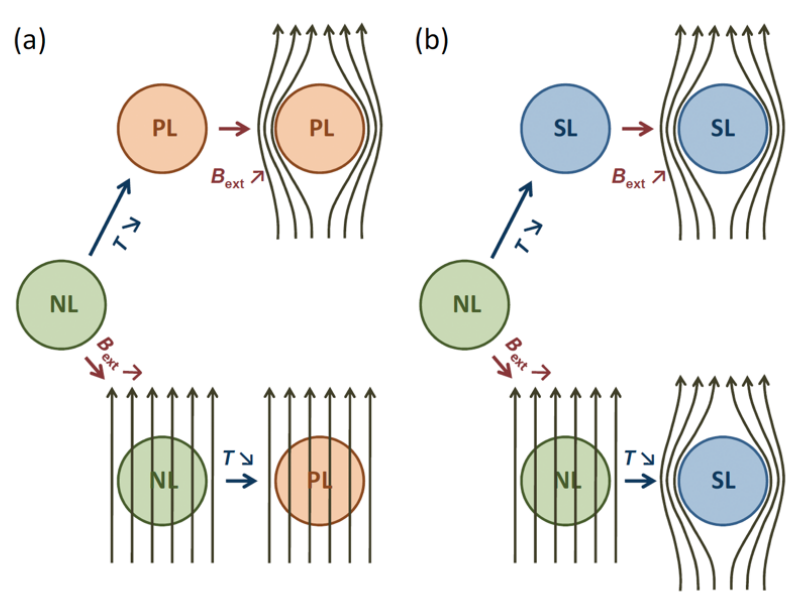
\includegraphics[width=0.5\textwidth]{Plots/MO_Effekt.png}
	\caption{Dargestellt ist hier der Unterschied zwischen (a) einem Normalleiter (NL) und (b) einem Supraleiter (SL). Jeweils wird der Leiter unter die kritische Temperatur herunter gek\"{u}hlt, bevor ein externes Magnetfeld $B_{ext}$ angelegt und nachdem $B_{ext}$ eingeschaltet wird. \cite{einleitung}}
	\label{abb:MOEffekt}
\end{SCfigure}


\paragraph{Kritisches Magnetfeld}
Wenn der, im letzten Abschnitt beschriebene Mei{\ss}ner-Och{\-}sen{\-}feld-Effekt (M.O.-Effekt) irreversibel w\"{a}re, dann m\"{u}sste der Supraleiter eine unendlich hohe Magnetfeldverdrängungsarbeit leisten k\"{o}nnen.
Da dies nicht der Fall ist, muss der M.O.-Effekt reversibel sein.
Das ist genau dann gegeben, wenn die Supraleitung durch ein externes B-Feld beziehungsweise durch ein kritisches B-Feld, $B_C$, zerst\"{o}rt wird.
Dies bedeutet im Einzelnen, dass die magnetische Flussdichte im Inneren des Supraleiters $B_I$ so lange gleich Null ist, wie $\mu_0H_{ext} \leq B_C(T)$ gilt.
Wie in Abbildung (\ref{abb:kritischesBFeld}a) zu sehen ist, nimmt $B_I$ proportional zum extern angelegten B-Feld zu, sobald $\mu_0H_{ext}$ den kritischen Wert von $B_C$ \"{u}berschritten hat.
Der Verlauf der Magnetisierung des Supraleiters ist in Abbildung (\ref{abb:kritischesBFeld}b) schematisch dargestellt.
Im ersten Bereich (schraffierte Fl\"{a}che) steigt die Magnetisierung linear nach der Gesetzm\"{a}{\ss}igkeit $-\mu_0M = \mu_0H_{ext} - B$ mit $B = 0$.
\"Uberschreitet das angelegte Magnetfeld den kritischen Wert des Supraleiters, nimmt $B = \mu_0H_{ext}$ an und die Magnetisierung bricht zusammen.
\begin{SCfigure}[1][!h]
	\centering
	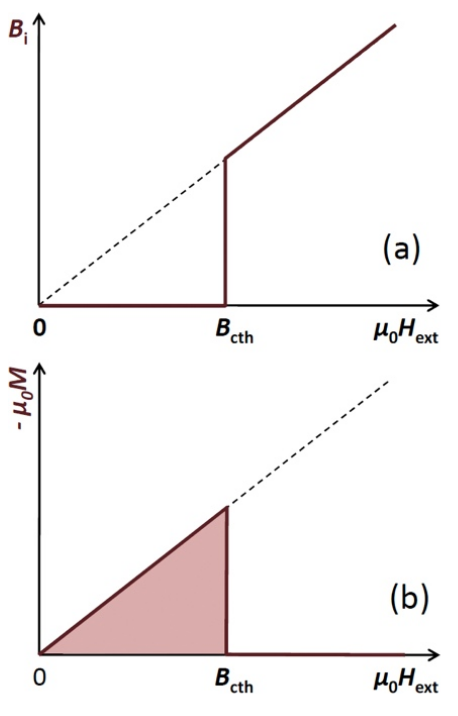
\includegraphics[width=0.35\textwidth]{Plots/kritischesBFeld.png}
 	\caption{In (a) ist die magnetische Flussdichte im Inneren eines Supraleiters dargestellt und in (b) ist die Magnetisierung eines Supraleiters als Funktion des externen Magnetfelds zu sehen. Hier bezeichnet $B_{cth}$ das kritische Magnetfeld. \cite{einleitung}}
	\label{abb:kritischesBFeld}
\end{SCfigure}
Das hier beschriebene Verhalten bezieht sich auf einen Supraleiter des Typs-I.
Und das kritische Magnetfeld ist zudem noch temperaturabh\"{a}ngig: $B_C = B_C(T)$.
Diese Abh\"{a}ngigkeit l\"{a}sst sich wie folgt ausdr\"{u}cken:
\begin{align*}
	B_C(T) = B_C(0) \left[ 1 - \left( \frac{T}{T_C} \right)^2 \right]
\end{align*}
$B_C(0)$ nimmt bei Supraleitern einige $10 \, $mT an.

\paragraph{Typ 2-Supraleiter}
\label{para:typ2}
Bisher wurde nur der Typ I-Supraleiter vorgestellt.
Bei einem Supraleiter des Typs-II gibt es noch einen \"{U}bergangsbereich zwischen der normalleitenden Phase und dem homogenen Supraleiter.
Somit gibt es auch zwei kritische Magnetfelder mit $B_{c,1} < B_{c,2}$.
Ist das angelegte Magnetfeld gr\"{o}{\ss}er als $B_{c,2}$ befindet sich der Supraleiter in der normalleitenden Phase.
Und unterhalb $B_{c,1}$ herrscht auf Grund des Mei{\ss}ner-Ochsenfeld-Effekts eine vollst\"andige Abschirmung des Magnetfeldes.
Es liegt ein homogener Supraleiter vor.
F\"{u}r den Fall, dass das angelegte Magnetfeld sich genau zwischen den beiden kritischen Magnetfeldern befindet, ist folgende Bedingung erf\"{u}llt: $B_{c,1} < B < B_{c,2}$, so liegt eine gemischte Phase vor.
In diesem Bereich bilden sich zun\"{a}chst zylinderf\"{o}rmige Flussschl\"{a}uche aus.
Diese werden immer gr\"{o}{\ss}er, bis sie das ganze Volumen des Leiters einnehmen.

\paragraph{Entropie und spezifische W\"{a}rme}
In Abbildung (\ref{abb:spezWaerme}) ist der Temperaturverlauf der spezifischen W\"{a}rme grafisch dargestellt.
In gelb der Verlauf eines normalleitenden Metalls, dieser steigt linear mit der Temperatur.
Im Gegensatz dazu verh\"{a}lt sich $C_s$, in Abbildung (\ref{abb:spezWaerme}) in blau dargestellt, f\"ur tiefe Temperaturen exponentiell.
Dieses Verhalten gibt einen eindeutigen Hinweis darauf, das im Anregungsspektrum eine Energiel\"ucke vorhanden sein muss.
Im Bereich der kritischen Temperatur gilt vor allem $C_n(T_C) < C_s(T_C)$.
\begin{figure}[hbtp]
	\centering
	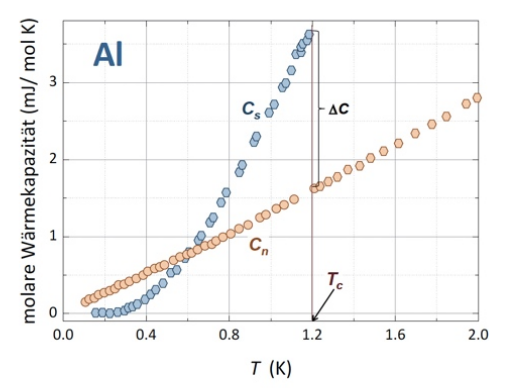
\includegraphics[width=0.55\textwidth]{Plots/spezWaerme.png}
	\caption{Vergleich der Temperaturverl\"{a}ufe der spezifischen W\"{a}rme von normalleitendem und supraleitendem Aluminium. \cite{einleitung}}
	\label{abb:spezWaerme}
\end{figure}


\paragraph{Die BCS-Theorie}
Ein Versuch, die theoretischen Hintergr\"unde eines Supraleiters zu verstehen, bietet die BCS-Theorie.
%Im Vergleich zum normalleiteden Zustand beschreibt der supraleitende Zustand den geordneter Zustand.
Zur heutigen Zeit ist es sicher, dass die Supraleitung durch die effektive Wechselwirkung der Elektronen untereinander verursacht wird.
Durch die effektive Coulomb-Anziehung der Elektronen wird der Fermi-See irgendwann unstabil.
So stellt sich ein neuer, energetisch g\"unstigerer Grundzustand ein.
Das Ganze l\"asst sich anhand von zwei Elektronen beispielhaft vorstellen.
Diese zwei Elektronen gehen auf Grund der anziehenden Wechselwirkung einen gebundenen Zustand ein, welcher als Cooper-Paar bezeichnet wird.
Dabei ist der mikroskopische Mechanismus hinter dieser chemischen Bindung bislang noch unklar.
In der BSC-Theorie wird die effektive anziehende Wechselwirkung durch die Elektronen-Phonon-Wechselwirkung beschrieben.
Wobei diese jedoch im Bereich von $30-40 \, $K liegt.
Weshalb damit zwar die Niedertemperatur-Supraleitung erkl\"art werden kann, jedoch nicht ganz die Hochtemperatur-Supraleitung.
Damit nun die zwei gedachten Elektronen ein Cooper-Paar bilden k\"onnen, m\"ussen sich diese Elektronen an der Fermikante aufhalten.
Zudem m\"ussen die beiden Elektronen einen umgekehrten Spin und einen entgegengesetzten Impuls besitzen.
Somit ist der Spin und der Impuls eines Cooper-Paares gleich Null.
Dies bedeutet, dass es sich bei Cooper-Paaren um Bosonen handelt, weshalb sie bei hinreichend tiefen Temperaturen kondensieren k\"onnen.
Au{\ss}erdem besitzen Bosonen eine gro{\ss}e r\"aumliche Ausdehnung.
Das Phonon in der Elektronen-Phonon-Wechselwirkung wird von dem einen Elektron erzeugt und innerhalb der Unsch\"arfe direkt wieder von dem zweiten Elektron des Cooper-Paares absorbiert.